\section{Desarrollo}
	\subsection{Construcción del sistema lineal}
	Dijimos que, dado un puente de $n$ secciones, consideraríamos un sistema de $4n$ ecuaciones y $4n$ variables, dónde (casi todas) éstas representan las fuerzas que ejercen los links sobre las juntas. Para esto, debimos numerar los links de alguna manera, para asociarlos con las variables del sistema. Veamos cómo construimos esto, y qué podemos deducir de ello en términos de la matriz.

Veamos el ejemplo de numeración, para el caso $n = 6$, de la figura \ref{fig:numeracion}:
\begin{figure}[!ht]
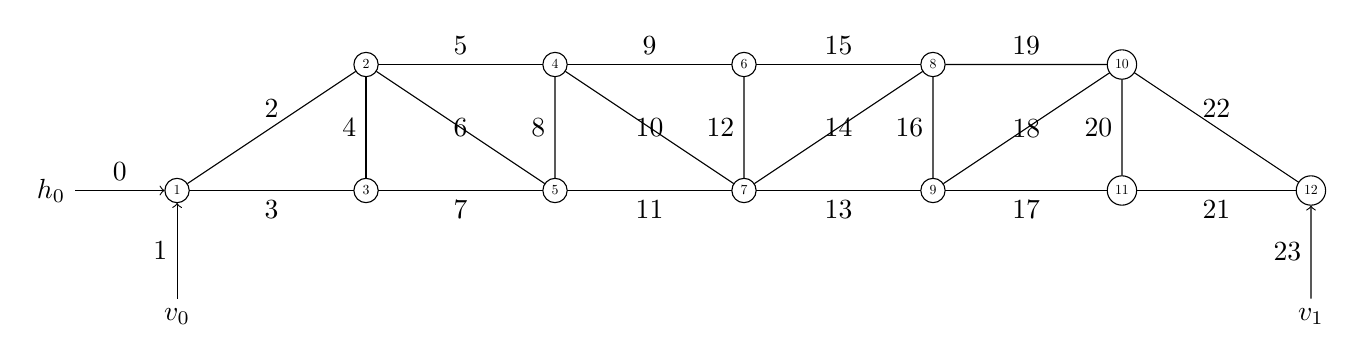
\begin{tikzpicture}[scale=0.8]

    \tikzset{nodestyle/.style={draw,shape=circle,scale=0.5}}
    \node[nodestyle] (p1) at ( 0, 0) {1}; 
    \node[nodestyle] (p2) at ( 3, 0) {3};
    \node[nodestyle] (p3) at ( 6, 0) {5};
    \node[nodestyle] (p4) at ( 9, 0) {7};
    \node[nodestyle] (p5) at ( 12, 0) {9};
    \node[nodestyle] (p6) at ( 15, 0) {11};
    \node[nodestyle] (p7) at ( 18, 0) {12};

    \node[nodestyle] (p8) at ( 3, 2) {2};
    \node[nodestyle] (p9) at ( 6, 2) {4};
    \node[nodestyle] (p10) at ( 9, 2) {6};
    \node[nodestyle] (p11) at ( 12, 2) {8};
    \node[nodestyle] (p12) at ( 15, 2) {10};

    \begin{scope}[every path/.style={-}]
        \draw (p1) -- (p2) node[below,midway]{$3$};
        \draw (p2) -- (p3) node[below,midway]{$7$}; 
        \draw (p3) -- (p4) node[below,midway]{$11$};
        \draw (p4) -- (p5) node[below,midway]{$13$};
        \draw (p5) -- (p6) node[below,midway]{$17$};
        \draw (p6) -- (p7) node[below,midway]{$21$};

        \draw (p8) -- (p9) node[above,midway]{$5$};
        \draw (p9) -- (p10) node[above,midway]{$9$};
        \draw (p10) -- (p11) node[above,midway]{$15$};
        \draw (p11) -- (p12) node[above,midway]{$19$};

        \draw (p1) -- (p8) node[above,midway]{$2$};
        \draw (p12) -- (p7) node[above,midway]{$22$};

        \draw (p2) -- (p8) node[left,midway]{$4$};
        \draw (p3) -- (p9) node[left,midway]{$8$};
        \draw (p4) -- (p10) node[left,midway]{$12$};
        \draw (p5) -- (p11) node[left,midway]{$16$};
        \draw (p6) -- (p12)node[left,midway]{$20$};

        \draw (p8) -- (p3) node[midway]{$6$};
        \draw (p9) -- (p4)node[midway]{$10$};
        \draw (p4) -- (p11)node[midway]{$14$};
        \draw (p5) -- (p12)node[midway]{$18$};
    \end{scope}  

    
    \node (v0) at ( 0, -2) {$v_0$};
    \node (v1) at ( 18, -2) {$v_1$};
    \node (h0) at ( -2, 0) {$h_0$};

    %\begin{scope}[every path/.style={-}]
        \draw[->] (v0) -- (p1) node[left,midway]{$1$};
        \draw[->] (v1) -- (p7) node[left,midway]{$23$};
        \draw[->] (h0) -- (p1)node[above,midway]{$0$};
    %\end{scope}

        % Nodos artificiales.
         
\end{tikzpicture}
\caption{Numeración propuesta, en el caso $n = 6$.}
\label{fig:numeracion}
\end{figure}

Antes que nada, observemos que dado que la cantidad de secciones es par, la estructura del puente resulta simétrica, con lo cual podemos establecer las siguientes correspondencias entre las dos mitades:
\begin{itemize}
	\item La fuerza $i$ a la izquierda, se corresponde con la $4n-i$ a la derecha.
	\item La junta $j$ a la izquierda arriba, se corresponde con la $2n-i$ a la derecha arriba.
	\item La junta $j$ a la izquierda abajo, se corresponde con la $2(n+1)-i$ a la derecha abajo.
\end{itemize}

\begin{figure}[!ht]\begin{center}
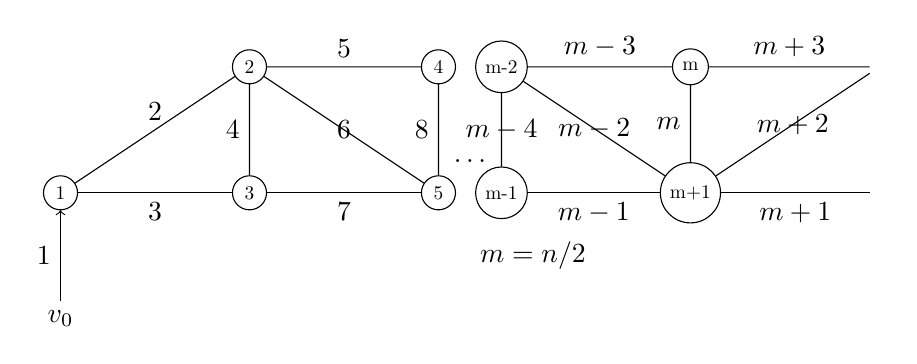
\begin{tikzpicture}[scale=0.8]

    \tikzset{nodestyle/.style={draw,shape=circle,scale=0.7}}
    \node[nodestyle] (p1) at ( 0, 0) {1}; 
    \node[nodestyle] (p2) at ( 3, 0) {3};
    \node[nodestyle] (p3) at ( 6, 0) {5};
    \node[nodestyle] (p33) at ( 7, 0) {m-1};
    \node[nodestyle] (p4) at ( 10, 0) {m+1};
    \node (p5) at ( 13, 0) {};

    \node[nodestyle] (p8) at ( 3, 2) {2};
    \node[nodestyle] (p9) at ( 6, 2) {4};
    \node[nodestyle] (p99) at ( 7, 2) {m-2};
    \node[nodestyle] (p10) at ( 10, 2) {m};
    \node (p11) at ( 13, 2) {};
    
    \node(pDots) at (6.5,0.5) {$\dots$};
    
    \begin{scope}[every path/.style={-}]
        \draw (p1) -- (p2) node[below,midway]{$3$};
        \draw (p2) -- (p3) node[below,midway]{$7$}; 
        \draw (p33) -- (p4) node[below,midway]{$m-1$};
        \draw (p4) -- (p5) node[below,midway]{$m+1$};


        \draw (p8) -- (p9) node[above,midway]{$5$};
        \draw (p99) -- (p10) node[above,midway]{$m-3$};
        \draw (p10) -- (p11) node[above,midway]{$m+3$};

        \draw (p1) -- (p8) node[above,midway]{$2$};

        \draw (p2) -- (p8) node[left,midway]{$4$};
        \draw (p3) -- (p9) node[left,midway]{$8$};
        \draw (p33) -- (p99) node[midway]{$m-4$};        
        \draw (p4) -- (p10) node[left,midway]{$m$};

        \draw (p8) -- (p3) node[midway]{$6$};
        \draw (p99) -- (p4)node[midway]{$m-2$};
        \draw (p4) -- (p11)node[midway]{$m+2$};
    \end{scope}  

    
    \node (v0) at ( 0, -2) {$v_0$};
    \node (aclaracion) at ( 7.5, -1) {$m = n/2$};

    %\begin{scope}[every path/.style={-}]
        \draw[->] (v0) -- (p1) node[left,midway]{$1$};
    %\end{scope}

        % Nodos artificiales.
         
\end{tikzpicture}
\caption{Numeración en el caso general, para la mitad izquierda.}
\label{fig:mediaNumeracion}
\end{center}
\end{figure}

Observemos que el caso complicado para la numeración de las fuerzas está dado por la cantidad variable (según $n$) de los links verticales interiores (es decir, aquellos que no son adyacentes ni a juntas consideradas extremos ($1$, $2$ ó $3$) ni a las juntas centrales. Las numeramos como $2p$ y $2p+1$, con $2 \leq p < n/2$, lo que nos produjo los siguientes resultados, que exponemos en el caso general. Esto se puede verificar fácilmente si tomamos el primero de ellos para establecer la relación entre las fuerzas y las juntas, e incrementamos en $4$ la numeración de cada fuerza tantas veces como links nos hayamos alejado del primero. Para la mitad derecha, resolvemos las relaciones de simetría explicadas anteriormente. Los cuatro casos posibles se muestran en la figura \ref{fig:juntasInt}.

\begin{figure}[!ht]
        \centering
        \begin{subfigure}[b]{0.24\textwidth}
                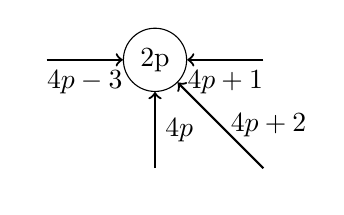
\begin{tikzpicture}[scale=0.5]

    \tikzset{nodestyle/.style={draw,shape=circle}}
    \node (p3) at ( 6, 0) {};
    \node (p4) at ( 9, 0) {};

    \node (p8) at ( 3, 3) {};
    \node[nodestyle] (p9) at ( 6, 3) {2p};
	\node (p10) at (9,3) {};

    \begin{scope}[every path/.style={->,thick}]
    	\draw (p8) -- (p9)node[midway,below]{$4p-3$}; 
        \draw (p3) -- (p9)node[midway,right]{$4p$};
        \draw (p4) -- (p9)node[midway,right]{$4p+2$};
		\draw (p10) -- (p9)node[midway,below]{$4p+1$};
    \end{scope} 
\end{tikzpicture}

                \caption{Junta superior izquierda}
                \label{fig:juntasupizq}
        \end{subfigure}
        \begin{subfigure}[b]{0.24\textwidth}
                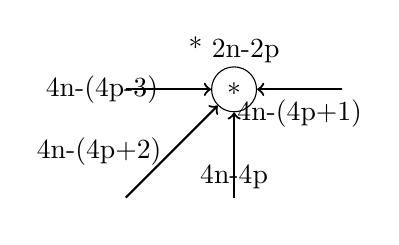
\begin{tikzpicture}[scale=0.5]

    \tikzset{nodestyle/.style={draw,shape=circle}}
    \node (p3) at ( 6, 0) {};
    \node (p4) at ( 3, 0) {};

    \node (p8) at ( 3, 3) {};
    \node(p99) at (6,4) {* 2n-2p};
    \node[nodestyle] (p9) at ( 6, 3) {$*$};
	\node (p10) at (9,3) {};

    \begin{scope}[every path/.style={->,thick}]
    	\draw (p8) -- (p9)node[midway,left]{4n-(4p-3)}; 
        \draw (p3) -- (p9)node[midway,below]{4n-4p};
        \draw (p4) -- (p9)node[midway,left]{4n-(4p+2)};
		\draw (p10) -- (p9)node[midway,below]{4n-(4p+1)};
    \end{scope} 
\end{tikzpicture}

                \caption{Junta superior derecha}
                \label{fig:juntasupder}
        \end{subfigure}
        \begin{subfigure}[b]{0.24\textwidth}
                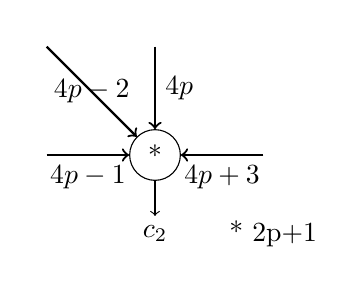
\begin{tikzpicture}[scale=0.5]

    \tikzset{nodestyle/.style={draw,shape=circle}}
    \node (p2) at ( 3, 0) {};
    \node (p33) at (9,-2) {* 2p+1};
    \node[nodestyle] (p3) at ( 6, 0) {*};
    \node (p4) at ( 9, 0) {};

    \node (p8) at ( 3, 3) {};
    \node (p9) at ( 6, 3) {};

    \begin{scope}[every path/.style={->,thick}]
        \draw (p2) -- (p3)node[midway,below]{$4p-1$}; 
        \draw (p4) -- (p3)node[midway,below]{$4p+3$};

        \draw (p9) -- (p3)node[midway,right]{$4p$};
        \draw (p8) -- (p3)node[midway]{$4p-2$};

    \end{scope} 
    \node (c2) at ( 6, -2) {$c_2$};

        \draw[->] (p3) -- (c2);
\end{tikzpicture}

                \caption{Junta inferior izquierda}
                \label{fig:juntainfizq}
        \end{subfigure}
        \begin{subfigure}[b]{0.24\textwidth}
                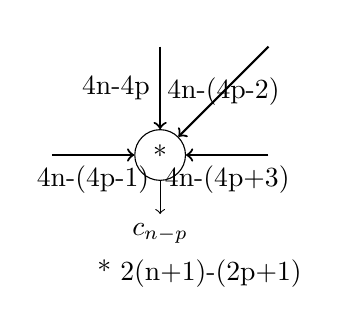
\begin{tikzpicture}[scale=0.5]

    \tikzset{nodestyle/.style={draw,shape=circle}}
    \node (p2) at ( 3, 0) {};
   \node(p33) at (7,-3) {* 2(n+1)-(2p+1)};
    \node[nodestyle] (p3) at (6, 0) {*};
    \node (p4) at ( 9, 0) {};

    \node (p8) at ( 9, 3) {};
    \node (p9) at ( 6, 3) {};

    \begin{scope}[every path/.style={->,thick}]
        \draw (p2) -- (p3)node[midway,below]{4n-(4p-1)}; 
        \draw (p4) -- (p3)node[midway,below]{4n-(4p+3)};

        \draw (p9) -- (p3)node[midway,left]{4n-4p};
        \draw (p8) -- (p3)node[midway]{4n-(4p-2)};

    \end{scope} 
    \node (c2) at ( 6, -2) {$c_{n-p}$};

        \draw[->] (p3) -- (c2);
\end{tikzpicture}

                \caption{Junta inferior derecha}
                \label{fig:juntainfder}
        \end{subfigure}
        \caption{Juntas interiores}\label{fig:juntasInt}
\end{figure}

Veamos cómo se traduce lo anterior a las ecucaciones de un sistema en general. Para el desarrollo, supondremos que contamos con por lo menos cuatro secciones (el caso para $n = 2$ es un caso particular pequeño que no requiere tanta generalidad). Sabemos que necesitamos escribir dos ecuaciones por cada junta $1 \leq j \leq 2n$, y que cada una tiene su simétrica. Por lo tanto, proponemos utilizar las ecuaciones $2(j-1)$, $2(j-1)+1$ si la junta está a la izquierda, y $4n-2j$, $4n-2j+1$ para su simétrica a derecha, siempre comenzando por la ecuación horizontal. Debimos descomponer la fuerza ejercida por los links oblicuos en las componentes verticales y horizontales, para lo que calculamos el seno y el coseno del ángulo con el que éstos inciden, simplemente como la proporción entre la longitud de la sección vertical (resp. horizontal) y la longitud del link oblicuo (lo que en las ecuaciones aparece como $\seno$ y $\cos$, respectivamente). Además, supusimos que todos los links están en tensión (es decir, las 
fuerzas actúan siempre en el sentido hacia las juntas), con lo cual valores negativos indicarán que en realidad, en la estructura están en compresión; también decifinimos como sentido positivo hacia la derecha y hacia abajo. Luego, las figuras anteriores se traducen en:

Para los extremos (juntas $1$, $2$ y $3$ y sus simétricas):
\begin{align*}
	0:& & 0 &= x_0 - \cos x_2 - x_3   & 4n-2: & & 0 &=   x_{4n-3}+ \cos x_{4n-2} \\
	1:& & 0 &= - x_1 + \seno x_2   & 4n-1: & & 0 &= \seno x_{4n-2}  + x_{4n-1} \\
	\\
	2: & & 0 &=  \cos x_2 - x_4 - \cos x_6  &  4n-4: & &0 &= x_{4n-7} - x_{4n-3} \\
	3: & & 0 &= - \seno x_2 -  x_4 - \seno x_6 & 4n-3: & & 0 &= x_{4n-4}   \\
	\\
	4: & & 0 &=  x_3 - x_7  & 4n-6: && 0&=  \cos x_{4n-6} + x_{4n-5} - \cos x_{4n-2}\\
	5: & & -q_1 &= x_4 &  4n-5: && -q_{n-1} &= -\seno x_{4n-6} - x_{4n-4} - \seno x_{4n-2}
\end{align*}

Para el tramo del medio (juntas $m$ y $m+1$):
\begin{align*}
2n-2:& & 0 &= x_{2n-3} - x_{2n+3}  \\
2n-1:& & 0 &= -x_{2n}  \\
\\
2n: & & 0 &= x_{2n-1} + \cos x_{2n-2} - \cos x_{2n+2} - x_{2n+1}   \\
2n+1: & & -q_{n/2 -1} &= x_{2n} + \seno x_{2n-2} + \seno x_{2n+2}   
\end{align*}

Para las juntas interiores (juntas $2p$ y $2p+1$ con $2 \leq p < n/2$ y sus simétricas):

\begin{align*}
4p-2: & & 0 &=x_{4p-3} - x_{4p+1} - \cos x_{4p+2} & 4(n-p): & & 0 &= \cos x_{4(n-p)-2} + x_{4(n-p)-1} -  x_{4(n-p)+3}\\
4p-1: & &0 &= -x_{4p} - \seno x_{4p+2} & 4(n-p)+1: & & 0 &= -\seno x_{4(n-p)-2} - x_{4(n-p)} \\
\\
4p: & & 0 &= \cos x_{4p-2}  + x_{4p-1} - x_{4p+3}  & 4(n-p)-2: & & 0 &= x_{4(n-p)-3} + x_{4(n-p)+1} - \cos x_{4(n-p)+2} \\
4p+1: & &-q_{p} &= \seno x_{4p-2} +x_{4p} & 4(n-p)-1: & & -q_{n-p} &= x_{4(n-p)} + \seno x_{4(n-p)+2} \\
\end{align*}

Ahora que tenemos las ecuaciones escritas en términos genéricos, miremos las bandas de la matriz. Podemos deducir los valores de las bandas de las cotas para las diferencias entre los índices de las variables y las ecuaciones (si no hubiera diferencia, la matriz sería puramente diagonal). La banda superior (o derecha) es $6$ y se alcanza en la ecuación $2n-2$, mientras que la inferior (o izquierda) es $4$ y se alcanza en las ecuaciones $4n-4$, $4p+1$, $4(n-p)+1$. \footnote{Observemos que si la diferencia entre el número de ecuación y el número de variable es $p$, la banda resultante es $p+1$, si pensamos que una matriz diagonal tiene bandas $1$}



	\subsection{Representación de la matriz asociada al sistema}
Vimos, tal como lo habíamos adelantado en la introducción, que efectivamente la matriz asociada al sistema es una matriz con estructura de bandas, que el ancho de las bandas es constante con respecto al tamaño del sistema y que aún dentro de las bandas hay coeficientes nulos. En consecuencia, la matriz asociada al sistema es una matriz muy poco densa, con lo cual surge la idea de utilizar una representación que refleje esta propiedad para reducir el uso de memoria. La solución propuesta consiste en utilizar listas enlazadas para almacenar los elementos no nulos de cada fila. Dado que no almacenaremos los elementos nulos, cada elemento debe estar acompañado del índice que le corresponde dentro de la fila, y la lista ordenada por éstos de manera creciente, para que las operaciones entre filas se puedan realizar de manera eficiente. Las filas (listas) las almacenamos en un vector que se inicializa al crear la matriz, aún cuando éstas estén vacías. 

\subsubsection{Complejidad Espacial}
Por lo que dijimos, es claro que si $nZ(A)$ es la cantidad de elementos no nulos de la matriz $A \in \R^{n\times n}$, en memoria tenemos reservadas $\O(zN(A) + n)$ posiciones. En el caso particular del T.P., en el que la cantidad de elementos no nulos de cada fila están dentro de las bandas, y éstas están acotadas por $p+ (p+q) = F$, esta complejidad resulta $\O(nF)$. Teóricamente, dado que $F$ no depende de $n$, podemos decir que la complejidad espacial es lineal en la dimensión de la matriz. Además, en este caso, para puentes grandes (digamos, de más de 25 secciones), mientras la cantidad de ecuaciones es del orden de la centena, $F$ es considerablemente menor (un orden de magnitud, por lo menos), con lo cual efectivamente no es significativo en términos prácticos. En este aspecto, la estructura es notablemente mejor que la solución trivial del arreglo bidimensional, ya que, por un lado, tiene un grado de complejidad menor, y por otro, en ningún momento tiene reservada memoria que no necesite efectivamente.

\subsubsection{Complejidad Temporal}  
 En términos generales, sabemos que reemplazar un arreglo por una lista enlazada degrada automáticamente la performance del acceso aleatorio a los elementos. Esto es efectivamente así, dado que para acceder a un elemento cualquiera debemos iterar sobre los elementos de la fila hasta encontrarlo (o alcanzar un elemento con un índice mayor, lo que indica que el elemento buscado no está representado, con lo cual, el valor requerido es $0$). Sin embargo, en estas condiciones, acceder al primer elemento no nulo (o a cualquiera de sus anteriores) insume tiempo constante ya que para esto no es necesario iterar por los elementos de la lista, simplemente alcanza con acceder al primero. Veremos que éste es el único acceso ``aleatorio'' que realiza nuestro algoritmo, con lo cual, no representa un problema para nosotros.
 
Veamos ahora cómo resultan las operaciones por filas, en las que se basa nuestro algoritmo. Por un lado, para intercambiar dos filas, dado que las representaciones de éstas son completamente independientes en memoria, basta con intercambiarlas en el arreglo de filas de la matriz. Si pensamos que, en general, las listas se representan como un puntero al primer elemento, basta intercambiar los correspondientes a las filas involucradas, lo que insume tiempo constante. (Más allá de que la representación efectiva de las listas utilizadas por la biblioteca estándar que estamos utilizando sea más compleja que un único puntero, en cualquier caso, es una cantidad constante de información, con lo cual  el tiempo requerido para realizar el intercambio sigue siendo una cantidad constante.) Veamos ahora la operación que a una fila le suma un múltiplo de otra. Si conseguiéramos realizar esta operación en tiempo lineal, no estaríamos degradando la performance con respecto a la representación con arreglos. Veremos que 
efectivamente podemos conseguir esto, utilizando una estrategia muy similar al paso \emph{merge} de \emph{Merge-Sort}. El pseudocódigo propuesto es el siguiente:
\begin{algorithm}
\caption{$F_i \gets F_i + k*F_t$}
\begin{algorithmic}
\State $itF_i := iteradorAlInicio(F_i)$
\State $itF_t := iteradorAlInicio(F_t)$
\While{$itF_i \neq fin(F_i)$ e $itF_t \neq fin(F_t)$}
	\If {$itF_i\rightarrow indice  < itF_t\rightarrow indice$}  
				\State $avanzar(itF_i)$ \Comment{El próximo elemento no nulo de $F_t$ es posterior al actual no nulo de $F_i$}
			\Else \If {$itF_i \rightarrow indice = itF_t \rightarrow indice$}  \Comment{Ambas filas tienen un elemento no nulo en la misma posición}
				\State $itF_i\rightarrow valor$ += $itF_t\rightarrow valor * k$
				\If {$itF_i \rightarrow valor \approx 0$}
					\State $eliminarActual(itF_i)$
				\Else
					\State $avanzar(itF_i)$
				\EndIf
				\State $avanzar(itF_t)$
			\Else \Comment{$F_t$ tiene un valor no nulo donde $F_i$ tiene un 0}
			%//itThis > itF, itThis es el primer valor que supera la posición del que estamos mirando en f.
				\State $F_i.insertarActual(itF_i, *itF_t)$
				\State $itF_i\rightarrow valor$ *= $k$
				\State $avanzar(itF_t)$
			\EndIf
\EndIf
\EndWhile
\While{$itF_t \neq fin(F_t)$}
		\State $F_i.agregarAlFinal(*itF_t)$ \Comment{Todavía quedan elementos para considerar en $F_t$}
		\State $F_i.\acute ultimo.valor$ *= $k$%\Comment{El pseudocódigo no se debería comentar}
\EndWhile
\end{algorithmic}
\end{algorithm}
 
 Observemos que el primer ciclo efectivamente ``intercala'' ordenadamente los elementos de $F_t$ adecuadamente multiplicados entre los de $F_i$ en caso de que alguna de las dos filas tenga un elemento nulo en la posición considerada (con lo cual, evita realizar operaciones aritméticas que involucren ceros), y en caso de que ambas filas cuenten con un elemento en la misma posición, almacena la suma correspondiente. En el caso que la suma introduzca un elemento nulo, éste es eliminado por el iterador. Realiza esto mientras existan elementos no nulos en ambas filas (pues cuando éstos se agotan en alguna, se alcanza el final de la fila invalidando la guarda del ciclo, ya que no almacenamos elementos nulos ). Si se agotaron los elementos de $F_t$, el segundo ciclo no se ejecuta, dejando inalterada la última porción de $F_i$, lo cual es correcto ya que las operaciones que realizaría sería sumar un $0$ a las posiciones no nulas del final de $F_i$. Por el contrario, si restan elementos en $F_t$ (pero no en $F_i$), simplemente hay que agregar éstos multiplicados por $k$ al final de $F_i$ (ya que 
correspondería con sumar éstos a ceros de $F_i$). Notemos dos cosas: por un lado, todas las operaciones que involucran elementos nulos no sólo no se computan, sino que se ignoran por completo, lo cual, para una matriz esparsa, representa una optimización no despreciable; por otro, en ningún momento el algoritmo depende de la estructura en bandas de la matriz, con lo cual funciona para matrices en general, resultando provechoso para matrices esparsas cualesquiera. Veremos que en el algoritmo de eliminación esto nos permite desentendernos de los valores de las bandas de la matriz, para los cuales, durante el transcurso del algoritmo no conocemos sus valores exactos sino cotas, nuevamente evitándonos computar operaciones triviales sin necesidad de predecir qué coeficientes son nulos.
 
 Veamos, finalmente, que este algoritmo tiene la complejidad deseada. Todas las operaciones que realiza las podemos suponer de costo constante ya que involucran avanzar en un paso o desreferenciar los iteradores u operaciones aritméticas. Además, como la condición de corte de los ciclos está dada por alcanzar el final de la listas y nunca retrocedemos los iteradores, podemos afirmar que en el peor caso, entre los dos ciclos, se producen tantas iteraciones como elementos no nulos tuvieran éstas. Con lo cual, realizamos $\O(nZ(F_i) + nZ(F_t))$, que en el caso general puede ser tan malo como $2n$, lo que resulta en la complejidad lineal que buscábamos. Además, en el caso particular del T.P., como vimos en lo referente a la complejidad espacial, este valor está acotado por $F = 2p+q$, que no sólo es constante con respecto a $n$, sino significativamente menor que éste. Luego, teóricamente podemos afirmar que esta operación tiene costo constante en función de $n$, y prácticamente, que su costo es un valor menor 
dentro del algoritmo de eliminación.

  Es necesario aclarar que cuando se eliminan elementos utilizando el iterador ($eliminarActual(itF_i)$), éste no se indefine puesto que se utiliza el método $\emph{erase}$ de la estructura estándar $\emph{list}$. Este método nos devuelve un iterador apuntando al elemento siguiente del eliminado, asegurándonos que este iterador no se indefine, y en el caso que se elimina el último elemento, simplemente retorna lo mismo que el método $\emph{end}$ del contenedor.

\subsection{Algoritmo de Resolución}
Como dijimos, utilizaremos el método de Eliminación de Gauss con pivoteo parcial para conseguir una matriz triangular superior cuyo sistema asociado sea equivalente al planteado al comienzo. En este paso aprovecharemos el hecho de contar con una matriz banda (tanto al comienzo como en cada paso del método) para acotar la búsqueda del pivote. Básicamente, si estamos en la iteración $j$ésima, necesitamos anular la $j$ésima columna de la matriz, para las filas inferiores a la $j$ésima. Recordando la definición de matriz banda, sabemos que $a_{i,j} = 0$ cuando $j \leq i-p$, o lo que es equivalente, cuando $i \geq j+p$, con lo cual sólo tiene sentido buscar el pivote en las filas $j < i < j+p$. Para el resto del algoritmo, no introdujimos modificaciones. En pseudocódigo:
 \begin{algorithm}
\caption{$triangular(A, b, bandaInferior)$}
\begin{algorithmic}
\For {$j$ desde $1$ hasta $n$}
	\State $ultimaFila := min(n, j+bandaInferior)$
    \State $i := buscarPivote(A, j+1, ultimaFila)$
        \If{$i \neq j$}
            \State $A.intercambiarFilas(i, j)$
			\State $b.intercambiarCoords(i,j)$
        \EndIf
     \State $pivote := A[j, j]$
     \For {$i$ desde $j+1$ hasta $ultimaFila$}   
        \State $a_{i,j} := A[i,j]$ %//(j,i) es el elemento a anular en la fila j. //es nulo, o es el primero no nulo :)
        \If {$a_{i,j} \not \approx 0$} 
	            \State $multiplicador := a_{i,j} / pivote$
	            \State $A.sumarMultiploDeFila(i, j, -multiplicador)$
	            \State $b[i]$ -= $b[j]*multiplicador$
	     \EndIf
      \EndFor
\EndFor
\end{algorithmic}
\end{algorithm}

El pseudocódigo expuesto corresponde a la implementación del método de Eliminación de Gauss con pivoteo sin mayores modificaciones. Como dijimos, la única diferencia está en la operación $buscarPivote$, que está restringida a las filas donde no podemos asegurar que no haya coeficientes nulos. La implementación de ésta es una búsqueda trivial de máximo módulo entre los elementos $a_{i,j}$, donde $i$ pertenece al rango explicado anteriormente y $j$ es la columna correspondiente a la iteración.
 
 Analicemos su complejidad. Sabemos que en el caso general, este método tiene complejidad $\O(n^3)$, veamos cómo lo afecta las reducciones aplicadas. Observemos las cotas: por un lado, como vimos antes, $ultimaFila - (j+1) \leq p < 2p+q = F$, con lo cual, tanto el segundo ciclo como la búsqueda del pivote, iteran a lo sumo esta cantidad de veces; el resto de las operaciones involucradas tienen costo constante, a excepción de $sumarMultiploDeFila$, que como vimos, tiene complejidad $\O(F)$. Esto es claro, salvo para los accesos a elementos de la matriz para los que, como dijimos al comienzo, no podemos garantizar siempre su ejecución en tiempo constante. Sin embargo, por cómo funciona el algoritmo, en la iteración $j$ésima en las columnas $j' <j$ ya se ha producido la eliminación, con lo cual, el primer elemento no nulo de las filas consideradas aparece, por lo menos, en la posición $j+1$. En estas condiciones, siempre estamos preguntando por el primer elemento no nulo de la fila (tanto en el valor de 
$pivote$ y $a_{i,j}$, como dentro de $buscarPivote$, lo que nos permite afirmar que, efectivamente, estas operaciones tienen costo constante. Luego, cada iteración realiza las siguientes cantidades de operaciones: $\O(F)$ para buscar el pivote, $\O(F)$ veces suma de dos filas, lo que tiene costo $\O(F)$, y una cantidad constante de otras operaciones también constantes. Luego, el cuerpo del ciclo insume $\O(F^2)$ operaciones, y por lo tanto, todo el algoritmo tiene complejidad $\O(nF^2)$. Como antes, suponiendo $F$ una constante acotada, asintóticamente el algoritmo de eliminación se realiza en tiempo lineal.  En la práctica, la relación entre $F^2$ y $n$ puede resultar más significativa que en los casos anteriores, pero si comparamos $nF^2$ contra $n^3$ estaríamos comparando $F^2$ contra $n^2$, donde, si $F$ es significativamente menor que $n$, esto resulta todavía más a favor de $F$.
 
 Una vez triangulada la matriz despejamos los valores de las variables utilizando el clásico algoritmo de \emph{backward substitution}. Para aprovechar la representación esparasa de la matriz, utilizamos un iterador reverso en cada fila.
 
 \begin{algorithm}[!h]
\caption{$despejar(A, b)$}
\begin{algorithmic}
\State $solucion[n] := 0 \dots 0$
\For {$i$ desde $n$ hasta $1$}
	\State $solucion[i] := b[i]$
	\State $itF = iteradorReverso(A.fila(i))$
     \While {$itF \neq principio(A.fila(i))$ e $itF \rightarrow indice > i$}   
	        \State $solucion[i]$ -= ($itF \rightarrow valor) * solucion[itF \rightarrow indice]$
	        \State $retroceder(itF)$
      \EndWhile
      		\State $solucion[i]$ /= $A[i,i]$
\EndFor
\end{algorithmic}
\end{algorithm} 
 
 Al igual que en el análisis de los casos anteriores, vemos que todas las operaciones involucradas en el algoritmo tienen costo constante (aún el acceso $A[i,i]$). El ciclo principal se repite $n$ veces, y el ciclo interior itera tantas veces como elementos no nulos tenga la fila luego de su diagonal. Es decir, a lo sumo el ancho de la banda superior, que es $p+q < 2p+q = F$. Luego, el costo de despejar las variables del sistema es $\O(nF)$, para el que, con los mismos argumentos que antes, podemos afirmar que es lineal y eficiente.
 
\subsection{Heurística}
  El algoritmo anterior permite calcular las fuerzas ejercidas por cada link en el puente, y por ende, la fuerza máxima en módulo. Luego, dada la fuerza máxima que pueden ejercer los links, podemos saber si el puente es o no seguro. Si el puente no es seguro, proponemos un método heurístico para colocar pilares auxiliares en el puente para luego analizar la seguridad del puente original, analizando la seguridad de las dos estructuras generadas por la inserción del pilar. Además de la inserción de pilares, el método propuesto calcular el costo total que demanda estas inserciones. \\
  
  A continuación, detallamos el algoritmo heurístico:
  
\begin{algorithm}[H]
\caption{$calcuarCostoTotal(puente)$}
\begin{algorithmic}
\State $costo\_estructura, cant\_pilares := calcularCostoEstructura(puente)$ \\
\Return $costo\_estructura * (cant\_pilares-1) * COSTO\_PILAR\_UNITARIO$
\end{algorithmic}
\end{algorithm}

\begin{algorithm}[H]
 \caption{$calcularCostoEstructura(puente)$}
 \begin{algorithmic}
  \State $costo\_estructura := 0$
  \State $cant\_pilares := 0$
  \State $resolverPuente(puente)$
  \If {el puente no es seguro}
  	\If{ $n > 2$} \Comment{El puente se puede seguir subdividiendo}
   			 \State $junta := elegirJunta(puente)$
    		\State $sub\_estructura\_1, sub\_estructura\_2 := generarSubEstructuras(junta)$
    		\State $costo\_sub_estructura\_1, cant\_pilares\_1 := calcularCostoEstructura(sub\_estructura\_1)$
    		\State $costo\_sub\_estructura\_2, cant\_pilares\_2 := calcularCostoEstructura(sub\_estructura\_2)$
    		\State $costo\_estructura += costo\_sub\_estructura\_1+costo\_sub\_estructura\_2$
    		\State $cant\_pilares += cant\_pilares\_1 + cant\_pilares\_2 + 1$
    \Else 
    		\State $costo\_estructura := +\infty$ 
    		\State $cant\_pilares := -1$ \Comment{La heurística no puede asegurar el puente.}
    \EndIf
  \Else
    \State $costo\_estructura := puente.calcularCostoParcial()$
  \EndIf \\
  \Return $costo\_estructura, cant\_pilares$    
 \end{algorithmic}
\end{algorithm}

  
Las clave de esta heurística reside en la elección de la junta, debajo de la cual se colocará un pilar. Optamos por elegir la junta más cercana al link sobre el cual se ejerce la fuerza máxima en módulo. Esta decisión intenta, mediante la inserción de un  pilar, relajar la fuerza que se genera alrededor de la junta donde se ejerce la fuerza más grande en módulo. Por otro lado, para elegir la junta tenemos en cuenta que se respete la simetría de las subestructuras generadas. En cuanto a la generación de las subestructuras, sólo hay que calcular el nuevo span para cada una. De esta manera, se van calculando los costos parciales de las subestructuras recursivamente así como también la cantidad de pilares utilizados, para finalmente realizar el cálculo del costo total en base a los costos parciales y la cantidad total de pilares insertados para asegurar la seguridad del puente. \\
